\documentclass{article}
\usepackage[utf8]{inputenc}
\usepackage{amsmath}
\usepackage{listings}
\usepackage{geometry}
\usepackage{graphicx}
\usepackage{appendix}
\usepackage{subfig}
\usepackage{gensymb}
\usepackage{cancel}
\usepackage{physics}
\usepackage{empheq}
\usepackage{wrapfig}
\usepackage[colorlinks=true]{hyperref}
\usepackage{xcolor}
\definecolor{codegreen}{rgb}{0,0.6,0}
\definecolor{codegray}{rgb}{0.5,0.5,0.5}
\definecolor{codepurple}{rgb}{0.58,0,0.82}
\definecolor{backcolour}{rgb}{0.95,0.95,0.92}
\lstdefinestyle{mystyle}{
    backgroundcolor=\color{backcolour},   
    commentstyle=\color{codegreen},
    keywordstyle=\color{magenta},
    numberstyle=\tiny\color{codegray},
    stringstyle=\color{codepurple},
    basicstyle=\ttfamily\footnotesize,
    breakatwhitespace=false,         
    breaklines=true,                 
    captionpos=b,                    
    keepspaces=true,                 
    numbers=left,                    
    numbersep=5pt,                  
    showspaces=false,                
    showstringspaces=false,
    showtabs=false,                  
    tabsize=2
}

\lstset{style=mystyle}

\title{Second Midterm}
\author{Simen Løken}
\date{November 2024}

\begin{document}

\maketitle
\renewcommand{\thesection}{Problem \arabic{section}}
\renewcommand{\thesubsection}{\alph{subsection})}
\section*{Contents}
This midterm contains Problem 1) through 7).\newline
Everything is answered (unless I missed something) with the exception of the comparison in Problem 6) with the results of Problem 3).
\newline
Repository with all code is at \href{https://github.com/simloken/FYS4480}{https://github.com/simloken/FYS4480}, wherein we have \texttt{main.py}, which contains functions for solving problem 2, 3, 5 and 7 respectively.
\section{}
With the definitions given in the midterm, we have then that:
\begin{equation*}
    \hat P _p ^+ = a_{p+}^\dagger a_{p-}^\dagger
\end{equation*}
\begin{equation*}
    \hat P _p^- = a_{p-} a_{p+}
\end{equation*}
and the spin operators:
\begin{equation*}
    \hat S_z = \frac{1}{2} \sum_{p\sigma} \sigma a_{p \sigma}^\dagger a_{p \sigma}
\end{equation*}
\begin{equation*}
    \hat S^2 = \hat S_z^2 + \frac{1}{2} \left(\hat S_+ \hat S_- + \hat S_- \hat S_+ \right)
\end{equation*}
where
\begin{equation*}
    \hat S_\pm = \sum_p a_{p\pm}^\dagger a_{\mp}
\end{equation*}
We need also a number operator $\hat N$ such that:
\begin{equation*}
    \hat N_{p \sigma} = a_{p \sigma}^\dagger a_{p\sigma}
\end{equation*}
which also means:
\begin{equation*}
    \hat H_0 = \xi \sum_{p \sigma} (p - 1) a_{p \sigma}^\dagger a_{p\sigma} = \xi \sum_{p \sigma} (p-1) \hat N_{p \sigma}
\end{equation*}
We now check that the commutation relations between the unperturbed Hamiltonian and $\hat S_z$. We have then that:
\begin{equation*}
    \left[\hat H_0, \hat S_z \right] = \frac{1}{2} \sum_{p\sigma} (p-1) \sum_{q \mu} \mu \left[a_{p\sigma}^\dagger a_{p \sigma}, a_{q \mu}^\dagger a_{q \mu} \right]
\end{equation*}
We recognize the latter sum as two number operators $N$, respectively $N_{p\sigma}$ and $N_{p\mu}$, which commute, meaning that:
\begin{equation}
    \left[ \hat H_0, \hat S_z \right] = 0
\end{equation}
Moving now onto the total spin $\hat S^2$ with the unperturbed Hamiltonian, which is defined as:
\begin{equation*}
    \left[ \hat H_0, \hat S^2 \right] = \left[\hat H_0, S_Z^2 \right] + \left[\hat H_0, \frac{1}{2} \left(\hat S_+ \hat S_- + \hat S_- \hat S_+\right) \right] = 0 + \left[\hat H_0, \frac{1}{2} \left(\hat S_+ \hat S_- + \hat S_- \hat S_+\right) \right]
\end{equation*}
Note that the first term becomes 0 as we know $\hat S_z$ commutes with $\hat H_0$. We have then
\begin{equation*}
    \left[ \hat H_0, \hat S_z^2 \right] = \left[\hat H_0, \frac{1}{2} \left(\hat S_+ \hat S_- + \hat S_- \hat S_+\right) \right] = \frac{1}{2} \left( \left[\hat H_0, \hat S_+ \hat S_-\right] + \left[\hat H_0, \hat S_- \hat S_+ \right]\right)
\end{equation*}
rewritten as:
\begin{equation*}
    \left[ \hat H_0, \hat S_+ \hat S_- \right] = \frac{1}{2} \left( \left[\hat H_0, \hat S_+\right] \hat S_- + \hat S_+ \left[\hat H_0, \hat S_- \right] +  \left[\hat H_0, \hat S_-\right] \hat S_+ + \hat S_- \left[\hat H_0, S_+ \right]\right)
\end{equation*}
Here, we can employ a simple trick, since we know that $\hat H_0$ is hermitian, and that $\hat S_+$ is the hermitian adjoint of $\hat S_-$. As such, it follows that:
\begin{equation*}
    \left[\hat H_0, \hat S_+ \right] = \left[\hat H_0, \hat S_- \right] = 0
\end{equation*}
and therefore:
\begin{equation}
    \left[\hat H_0, \hat S^2 \right] = 0
\end{equation}
We move now onto the perturbation $\hat V$, first starting with $\hat S_z$. We have then:
\begin{equation*}
    \left[\hat V, \hat S_z \right] = - \frac{1}{2} g \sum_{pq} \left[a_{p+}^\dagger a_{p-}^\dagger a_{q-} a_{q+}, \hat S_z \right]
\end{equation*}
We note that $\hat V$ contains $\hat P$, and rewrite:
\begin{equation*}
    \left[\hat V, \hat S_z \right] = - \frac{1}{2} g \sum_{pq} \left[\hat P_p ^+ \hat P_q^-, \hat S_z \right]
\end{equation*}
from which we get:
\begin{equation*}
    \left[\hat V, \hat S_z \right] = - \frac{1}{2} g \sum_{pq} \hat P_p^+\left[\hat P_q^-, \hat S_z \right] + \left[P_p^+, \hat S_z \right] \hat P_q^-
\end{equation*}
Here we again employ the same trick as before. Since we know that $\hat S_z$ is hermitian, and that, similar to $S_\pm$, the hermitian adjoint of $P_p^+$ is $P_p^-$, we again use that we know these must commute, giving:
\begin{equation}
    \left[ \hat V, \hat S_z \right] = 0
\end{equation}
We now move onto the last commutation relation, that of $\left[ \hat V, \hat S^2 \right]$. We get:
\begin{equation*}
    \left[ \hat V, \hat S^2 \right] = \left[ \hat V, \hat S_Z^2 \right] + \frac{1}{2} \left(\left[ \hat V, \hat S_+ \hat S_-\right] + \left[ \hat V, \hat S_- \hat S_+ \right]\right)
\end{equation*}
\begin{equation*}
    \left[ \hat V, \hat S^2 \right] = 0 + \frac{1}{2} \left(\left[ \hat V, \hat S_+ \hat S_-\right] + \left[ \hat V, \hat S_- \hat S_+ \right]\right)
\end{equation*}
Sadly, we cannot employ the same trick as last time. Instead, we find respectively the commutations of $\left[P_p^+, S_+ \right]$ and $\left[P_p^-, S_- \right]$
\begin{equation*}
    \left[P_p^+, S_+ \right] = \left[a_{p+}^\dagger a_{p-}^\dagger, \sum_q a_{q+}^\dagger a_{q-} \right] = a_{p+}^\dagger \left[a_{p-}^\dagger, \sum_q a_{q+}^\dagger a_{q-} \right] + \left[a_{p+}^\dagger, \sum_q a_{q+}^\dagger a_{q-} \right] a_{p-}^\dagger
\end{equation*}
Summing now over everything, we find that every commutator besides $p=q$ are 0, meaning:
\begin{equation*}
    \left[P_p^+, S_+ \right] =
    \sum_q \left( a_{p+}^\dagger a_{q+}^\dagger \left[a_{p-}^\dagger, a_{q-}\right] +
    a_{p+}^\dagger \left[a_p{-}^\dagger, a_{q+}^\dagger \right] a_{q-} +
    a_{q+}^\dagger \left[a_{p+}^\dagger, a_{q-}\right] a_{p-} + 
    \left[a_{p+}^\dagger, a_{q+}^\dagger \right]a_{q-} a_{p-}
    \right)
\end{equation*}
Giving finally:
\begin{equation*}
    \left[\hat P_p, \hat S_+ \right] = 
    a_{p+}^\dagger a_{p+}^\dagger \left[a_{p-}^\dagger, a_{p-} \right] + 
    a_{p+}^\dagger \left[a_{p-}^\dagger, a_{p+}^\dagger \right] a_{p-} + 
    a_{p+}^\dagger \left[a_{p+}, a_{p-} \right] a_{p-} +
    \left[a_{p+}^\dagger a_{p+}^\dagger \right] a_{p-} a_{p-}
\end{equation*}
\begin{equation}
    \left[\hat P_p, \hat S_+ \right] = 0 \xrightarrow[]{} \left[ \hat V, \hat S^2 \right] = 0
\end{equation}
Note that I omitted the calculation of $\left[\hat P_p, S_- \right]$ (which is necessary for the result above to be true), but it is done the same way as that of our above calculations. \newline
Lastly, we were asked to find $\left[P_p^+, P_p^+\right]$:
\begin{equation}
    \left[P_p^+, P_p^+\right] = a_{p+}^\dagger a_{p-}^\dagger a_{p+}^\dagger a_{p-}^\dagger - a_{p+}^\dagger a_{p-}^\dagger a_{p+}^\dagger a_{p-}^\dagger = 0
\end{equation}
and $\left[P_p^-, P_p^-\right]$:
\begin{equation}
    \left[P_p^-, P_p^-\right] = a_{p-}^\dagger a_{p+}^\dagger a_{p-}^\dagger a_{p+}^\dagger - a_{p-}^\dagger a_{p+}^\dagger a_{p-}^\dagger a_{p+}^\dagger = 0
\end{equation}
\section{}
We define the ground state by:
\begin{equation*}
    | \Phi_0 \rangle = a_{1+}^\dagger a_{1-}^\dagger a_{2+}^\dagger a_{2-}^\dagger |0\rangle = \hat P_{1}^+ \hat P_{2}^+ |0\rangle
\end{equation*}
leading to the other Slater determinants:
\begin{equation*}
    | \Phi_1 \rangle = \hat P_1^+ \hat P_3^+ | 0 \rangle
\end{equation*}
\begin{equation*}
    | \Phi_2 \rangle = \hat P_1^+ \hat P_4^+ | 0 \rangle
\end{equation*}
\begin{equation*}
    | \Phi_3 \rangle = \hat P_2^+ \hat P_3^+ | 0 \rangle
\end{equation*}
\begin{equation*}
    | \Phi_4 \rangle = \hat P_2^+ \hat P_4^+ | 0 \rangle
\end{equation*}
\begin{equation*}
    | \Phi_5 \rangle = \hat P_3^+ \hat P_4^+ | 0 \rangle
\end{equation*}
Now onto finding the matrix. We must now find the contributions of generic states $\alpha, \beta, \gamma, \delta$ on $\hat H_0$ and $\hat V$ respectively. We start with $\hat H_0$:
\begin{equation*}
    \langle (\alpha) (-\alpha) (\beta) (-\beta)| \hat H_0 | (\gamma) (-\gamma) (\delta) (-\delta) \rangle = \sum_{p \sigma} (p - 1) \langle (\alpha) (-\alpha) (\beta) (-\beta)| \hat N_{p \sigma} | (\gamma) (-\gamma) (\delta) (-\delta) \rangle
\end{equation*}
We can then sum over $\sigma$ and get:
\begin{equation*}
    \langle (\alpha) (-\alpha) (\beta) (-\beta)| \hat H_0 | (\gamma) (-\gamma) (\delta) (-\delta) \rangle = 2 \sum_p (p - 1) (\delta_{p\gamma} + \delta_{p \delta}) \langle (\alpha) (-\alpha) (\beta) (-\beta) | (\gamma) (-\gamma) (\delta) (-\delta) \rangle
\end{equation*}
Employing then Wicks Theorem we find that:
\begin{equation}
     \langle (\alpha) (-\alpha) (\beta) (-\beta)| \hat H_0 | (\gamma) (-\gamma) (\delta) (-\delta) \rangle = 2 (r + 2 - 2)(\delta_{\alpha \gamma} \delta_{\beta \delta} + \delta_{\alpha \delta} \delta_{\beta \gamma})
\end{equation}
We do now the same for $\hat V$, resulting in:
\begin{equation}
    \langle (\alpha) (-\alpha) (\beta) (-\beta)| \hat V | (\gamma) (-\gamma) (\delta) (-\delta) \rangle = - \frac{1}{2} g (\delta_{\beta \delta} + \delta_{\beta \gamma} + \delta_{\alpha \delta} + \delta_{\alpha \gamma} )
\end{equation}
This gives rise to two matrices, where the columns correspond to the states $\Phi_0$ through $\Phi_5$:
\begin{equation*}
\hat H_0 = 
    \begin{bmatrix}
        2 & 0 & 0 & 0 & 0 & 0 \\
        0 & 4 & 0 & 0 & 0 & 0 \\
        0 & 0 & 6 & 0 & 0 & 0 \\
        0 & 0 & 0 & 6 & 0 & 0 \\
        0 & 0 & 0 & 0 & 8 & 0 \\
        0 & 0 & 0 & 0 & 0 & 10
    \end{bmatrix}
\end{equation*}
\begin{equation*}
\hat V = -\frac{g}{2}
    \begin{bmatrix}
        2 & 1 & 1 & 1 & 1 & 0 \\
        1 & 2 & 1 & 1 & 0 & 1 \\
        1 & 1 & 2 & 0 & 1 & 1 \\
        1 & 1 & 0 & 2 & 1 & 1 \\
        1 & 0 & 1 & 1 & 2 & 1 \\
        0 & 1 & 1 & 1 & 1 & 2
    \end{bmatrix}
\end{equation*}
Adding these together gives us the resulting matrix:
\begin{equation}
    \hat H = 
    \begin{bmatrix}
        2 - g & -\frac{g}{2} & -\frac{g}{2} & -\frac{g}{2} & -\frac{g}{2} & 0 \\
        -\frac{g}{2} & 4 - g & -\frac{g}{2} & -\frac{g}{2} & 0 & -\frac{g}{2} \\
        -\frac{g}{2} & -\frac{g}{2} & 6 - g & 0 & -\frac{g}{2} & -\frac{g}{2} \\
        -\frac{g}{2} & -\frac{g}{2} & 0 & 6 - g & -\frac{g}{2} & -\frac{g}{2} \\
        -\frac{g}{2} & 0 & -\frac{g}{2} & -\frac{g}{2} & 8 - g & -\frac{g}{2} \\
        0 & -\frac{g}{2} & -\frac{g}{2} & -\frac{g}{2} & -\frac{g}{2} & 10 - g
    \end{bmatrix}
\end{equation}
which when diagonalizing and varying $g$ gives us the plot:
\newpage
\begin{figure}[ht!]
    \centering
    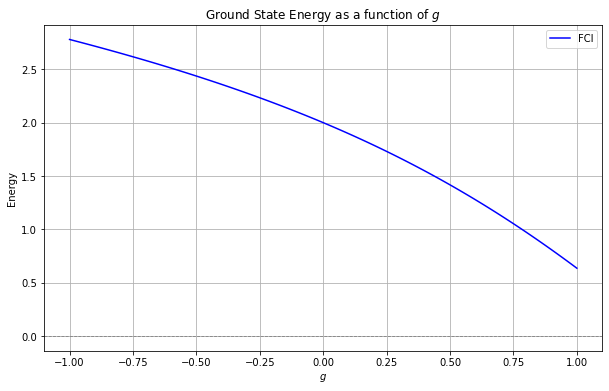
\includegraphics[width=0.6\linewidth]{exc2_1.png}
    \caption{A FCI plot as we vary the coupling strength $g$}
    \label{fig:enter-label}
\end{figure}
We note that the ground state energy decreases as we increase the coupling strength.
\newline
Additionally, we have the eigenvalues as a function of $g$:
\begin{figure}[ht!]
    \centering
    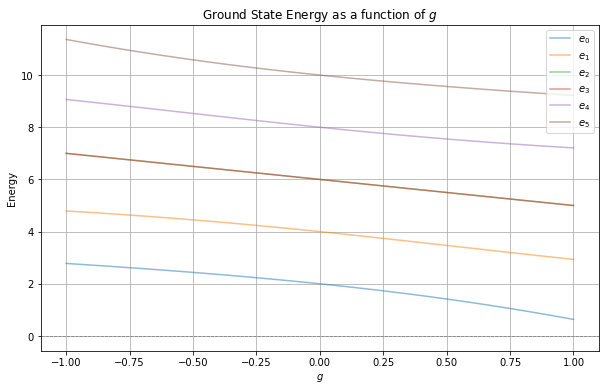
\includegraphics[width=0.6\linewidth]{exc2_2.png}
    \caption{An eigenvalue plot as we vary the coupling strength $g$}
    \label{fig:enter-label}
\end{figure}
\newline
We note that we only see five distinct lines, despite six eigenvalues. This is because we have degeneracy for $e_2, e_3$.
\newpage
\section{}
This means that we will have to remove the state(s) where the four particles are not in the two lowest orbits. This is only the case for the state $\Phi_5$, ie the final column (and row), giving us a new matrix:
\begin{equation}
    \begin{bmatrix}
        2 - g & -\frac{g}{2} & -\frac{g}{2} & -\frac{g}{2} & -\frac{g}{2}  \\
        -\frac{g}{2} & 4 - g & -\frac{g}{2} & -\frac{g}{2} & 0  \\
        -\frac{g}{2} & -\frac{g}{2} & 6 - g & 0 & -\frac{g}{2}  \\
        -\frac{g}{2} & -\frac{g}{2} & 0 & 6 - g & -\frac{g}{2}  \\
        -\frac{g}{2} & 0 & -\frac{g}{2} & -\frac{g}{2} & 8 - g  \\
    \end{bmatrix}
\end{equation}
and associated plot:
\begin{figure}[ht!]
    \centering
    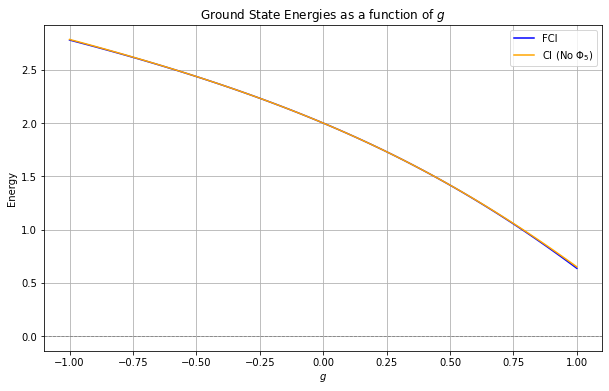
\includegraphics[width=0.5\linewidth]{exc3_1.png}
    \caption{A CI plot as we vary the coupling strength $g$, without $\Phi_5$}
    \label{fig:enter-label}
\end{figure}
\newline
A direct comparison between FCI and CI can be seen in the plot, but it can be a bit hard to see properly as they overlap so closely. We therefore look at the difference between the two plots instead:
\begin{figure}[ht!]
    \centering
    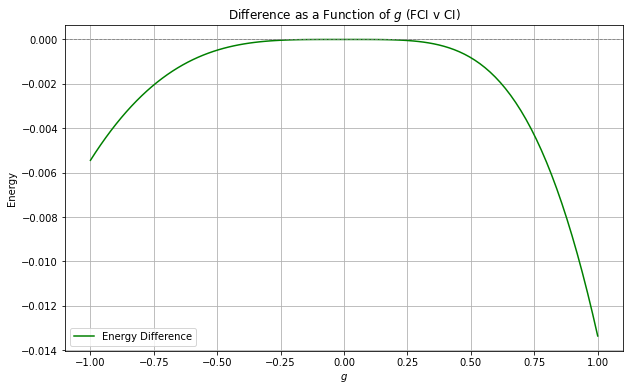
\includegraphics[width=0.5\linewidth]{exc3_2.png}
    \caption{A comparison of energy calculation between FCI and CI}
    \label{fig:enter-label}
\end{figure}
\newline
We see here that, although the differences are small, CI makes for a good method values of $g$ close to $0$. However, we see also a steep drop-off in accuracy as $g$ increases. This is perhaps related to the fact that we see the ground state energy increase sharply as we increase $g$ for the FCI method.
\section{}
We set the Fermi level to include the model space, $p = 1, 2$. This allows us to use the creation and annihilation operators $P_p^\pm$ to achieve to achieve the excluded space $p = 3, 4$. We move also to particle-hole formalism, where the fermi level states are indicated by $i,j,k ... \in \{1,2\}$ and the states above the fermi level are indicated by $a, b, c ... \in \{3,4\}$ \newline
For our reference state $|\Phi_0 \rangle$, the unperturbed Hamiltonian is given by:
\begin{equation*}
    \hat H_0  = \sum_{p \sigma} (p-1) a_{p_\sigma}^\dagger a_{p\sigma}
\end{equation*}
\begin{equation*}
    \sum_{p\sigma} (p-1) \hat N_{p\sigma} = \langle \Phi_0 | \hat H_0 | \Phi_0 \rangle + \sum_{p \sigma} (p - 1) \hat N_{p \sigma}
\end{equation*}
For the perturbation, we get:
\begin{equation*}
    \hat V = - \frac{1}{2}g \sum_{pq} \left(a_{p+}^\dagger a_{p-}^\dagger a_{q-} a_{q+} \right) - \frac{1}{2}g \sum_i \left( a_{p-}^\dagger a_{p-} + a_{p+}^\dagger a_{p+} \right) - \frac{1}{2} g \sum_i 1
\end{equation*}
Which in turn gives us the Fermi vacuum energy and $\hat H_0^N, \hat V^N$ from above:
\begin{equation*}
    E_0^\text{ref} = 2 \sum_i (i - 1) - \frac{1}{2} g M, \xrightarrow[]{M = 2} E_0^\text{ref} = 2 - g
\end{equation*}
Note that $M$ is the number of pair states \textit{below} the Fermi level.
\begin{equation*}
    \hat H_0^N = \sum_{p \sigma} \left((p -1) N_{p\sigma}\right) - \frac{1}{2} g \sum_{i \sigma} N_{i \sigma}
\end{equation*}
\begin{equation*}
    \hat V^N = -\frac{1}{2} \sum_{pq} \hat P_p^+ \hat P_q^-
\end{equation*}
We then have the Fock operator:
\begin{equation*}
    f_{pq} = \langle p | \hat f| q \rangle = \langle p | \hat H_0 | q \rangle + \sum_j \langle pj | \hat V | q j \rangle_{AS}
\end{equation*}
and it's second quantization:
\begin{equation*}
    \hat F = \sum_{pq} \langle p | \hat f | q \rangle a_p^\dagger a_q
\end{equation*}
Normally, this would be quite a troublesome calculation, but we can again employ a trick. We note that our Hamiltonian is 0 outside of the diagonal, meaning that $p=q$, and thus we only have one sum:
\begin{equation*}
    \hat F = \sum_p \langle p | \hat f | p \rangle a_p^\dagger a_p
\end{equation*}
which then, writing in normal order gives rise to:
\begin{equation*}
    \hat F \sum_p \langle p | \hat f | p \rangle a_p^\dagger a_p + \sum_i \langle i | \hat f | i \rangle
\end{equation*}
and finally the Canonical Hartree-Fock:
\begin{equation}
    \hat f | p \rangle = \sum_q \epsilon_{qp} | q\rangle
\end{equation}
\section{}
We use the equation found in the previous midterm (and/or lectures):
\begin{equation*}
        \sum_\beta h_{\alpha\beta}^{\mathcal{H}\mathcal{F}} C_{i\beta} = \epsilon_i C_{i \alpha}
\end{equation*}
While initially daunting, there are some things we can do to make this easier on ourselves. We note that, given the orthonormal basis, the one-body contribution $\hat h_0$ is actually entirely diagonal:
\begin{equation*}
    \langle \alpha | \hat h_0 | \beta \rangle = (\alpha - 1)\delta_{\alpha \beta}
\end{equation*}
Now we need to find the contribution from the two-body. Keeping in mind the restraints of our system, we note that a particular particle may be described by two quantum numbers, it's energy $e$ and its spin $\sigma$, thus a given configuration is just a sum over four quantum numbers, the energies and the spins of two particles respectively. We note also that the particles must \emph{share} energy level and that the spins \emph{have to} be opposite. With this in mind, we find again an entirely diagonal contribution.
\begin{equation*}
    \rho_{\alpha\beta}  \langle \alpha_+ \alpha_- |  V | \beta_+ \beta_- \rangle = -\frac{1}{2} g\rho_{\alpha\beta}
\end{equation*}
where the subscript $+, -$ indicate the spin.
\newline
As is customary, we assume $C_{i\alpha}^* = \delta_{i \alpha}$, or $C = I$. We note now that given $C$, the associated density matrix $\rho$ is diagonal, as is both the one-body and two-body contributions. Thus we already have a Hartree-Fock basis (!!!), and we don't really even need to do anything else. No explicit calculation or iteration is needed. The energy by our Hartree-Fock method then becomes a simple:
\begin{equation}
    E[\Phi_0^{\mathcal{H}\mathcal{F}}] = 2 - g
\end{equation}
in other words entirely linear with $g$. Perhaps this is "cheating" in the sense that we don't "solve" our Hartree-Fock model iteratively, but it is a welcome discovery!
\newline
Although not strictly necessary, we include here also the Hartree-Fock matrix:
\begin{equation*}
H^{\mathcal{H}\mathcal{F}} =
    \begin{bmatrix}
        0 - \frac{1}{2}g & 0 & 0 & 0 & 0 & 0 & 0 & 0 \\
        0 & 0 - \frac{1}{2}g & 0 & 0 & 0 & 0 & 0 & 0 \\
        0 & 0 & 1 - \frac{1}{2}g & 0 & 0 & 0 & 0 & 0 \\
        0 & 0 & 0 & 1 - \frac{1}{2}g & 0 & 0 & 0 & 0 \\
        0 & 0 & 0 & 0 & 2 & 0 & 0 & 0 \\
        0 & 0 & 0 & 0 & 0 & 2 & 0 & 0 \\
        0 & 0 & 0 & 0 & 0 & 0 & 3 & 0 \\
        0 & 0 & 0 & 0 & 0 & 0 & 0 & 3
    \end{bmatrix}
\end{equation*}
\newline
with the associated plot:
\newpage
\begin{figure}[ht!]
    \centering
    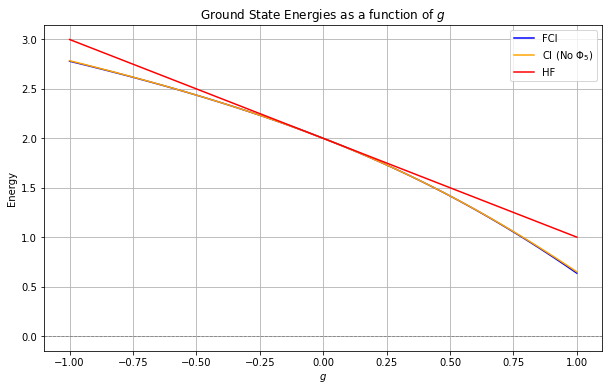
\includegraphics[width=0.6\linewidth]{exc5_1.png}
    \caption{Comparing the ground state energy calculation using both FCI, CI and HF.}
    \label{fig:enter-label}
\end{figure}
We note that HF is adequate in and around $g$, but as $g$ increases (or decreases), HF fails us. This isn't exactly much of a surprise, considering the linear nature of HF.
\newline
We again get a closer look with looking at the difference:
\begin{figure}[ht!]
    \centering
    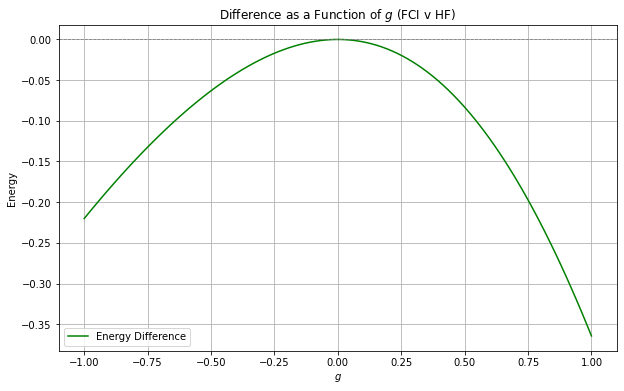
\includegraphics[width=0.6\linewidth]{exc5_2.png}
    \caption{The difference between FCI and HF}
    \label{fig:enter-label}
\end{figure}
\newline
Again, we see that HF is perfectly suitable when $g\approx 0$, but for any other value of $g$ we cannot realistically use this, especially given its linear nature.\newpage
We move now onto the Rayleigh-Schrödinger perturbation theory. The diagrams that contribute to the energy of the ground state are $1, 4, 5, 8 $ and $9$, as these are the only unbroken pairs. \newline
Starting from the "top", we have then:
\begin{equation}
    (1) \; \; \; \; \frac{1}{4} \sum_{abij} \frac{\langle ij | V | ab\rangle \langle ab | V | ij \rangle}{\epsilon_i + \epsilon_j - \epsilon_a - \epsilon_b} = \frac{1}{8} \sum_{ai} \frac{g^2}{i-a}
\end{equation}
\begin{equation}
    (4) \; \; \; \; \frac{1}{8} \sum_{abcdij} \frac{\langle ij | V | ab \rangle \langle ab | V | cd \rangle \langle cd | V | ij \rangle}{(\epsilon_i + \epsilon_j - \epsilon_a - \epsilon_b)(\epsilon_i \epsilon_j - \epsilon_c - \epsilon_d)} = -\frac{1}{32} \sum_{iac} \frac{g^3}{(i-a)(i-c)}
\end{equation}
\begin{equation}
    (5) \; \; \; \; \frac{1}{8} \sum_{abijkl} \frac{\langle kl | V | ij \rangle \langle ab | V | cd \rangle \langle cd | V | ij \rangle}{(\epsilon_i + \epsilon_j - \epsilon_a - \epsilon_b)(\epsilon_k \epsilon_l - \epsilon_a - \epsilon_b)} = -\frac{1}{32} \sum_{ika} \frac{g^3}{(i-a)(k-a)}
\end{equation}
\begin{equation}
    (8) \; \; \; \; -\frac{1}{2} \sum_{abijkl} \frac{\langle ij | V | ab \rangle \langle kl | V | ki \rangle \langle ab | V | lj \rangle}{(\epsilon_i + \epsilon_j - \epsilon_a - \epsilon_b)(\epsilon_i + \epsilon_k - \epsilon_a - \epsilon_b)} = \frac{1}{16} \sum_{ia} \frac{g^3}{(i-a)^2}
\end{equation}
\begin{equation}
    (9) \; \; \; \; -\frac{1}{2} \sum_{abcdij} \frac{\langle ij | V | ab \rangle \langle ca | V | cd \rangle \langle db | V | ij \rangle}{(\epsilon_i + \epsilon_j - \epsilon_a - \epsilon_b)(\epsilon_i + \epsilon_j - \epsilon_a - \epsilon_c)} = \frac{1}{16} \sum_{ia} \frac{g^3}{(i-a)^2}
\end{equation}
We then finally get our expression:
\begin{gather*}
    E^{(3)} = E^{(0)} + E^{(1)} + (1) + (4) + (5) + (8) + (9) = \\ 2 - g + \frac{1}{8} \sum_{ai} \frac{g^2}{i-a} - \frac{1}{32} \sum_{iac} \frac{g^3}{(i-a)(i-c)} -\frac{1}{32} \sum_{ika} \frac{g^3}{(i-a)(k-a)} + \frac{1}{16} \sum_{ia} \frac{g^3}{(i-a)^2} + \frac{1}{16} \sum_{ia} \frac{g^3}{(i-a)^2}
\end{gather*}
We evaluate and find:
\begin{equation*}
    E^{(3)} = 2 - g - \left(\frac{3g^2}{8} - \frac{g^2}{24} \right) + \left(\frac{53g^3}{576}\right) + \left(\frac{53g^3}{576}\right) + \left(\frac{29g^3}{288}\right) + \left(\frac{29g^3}{288}\right)
\end{equation*}
Simplifying to the polynomial:
\begin{equation}
    E^{(3)} = \frac{37g^3}{96} - \frac{5g^2}{12} - g + 2
\end{equation}
which we can plot:
\newpage
\begin{figure}[ht!]
    \centering
    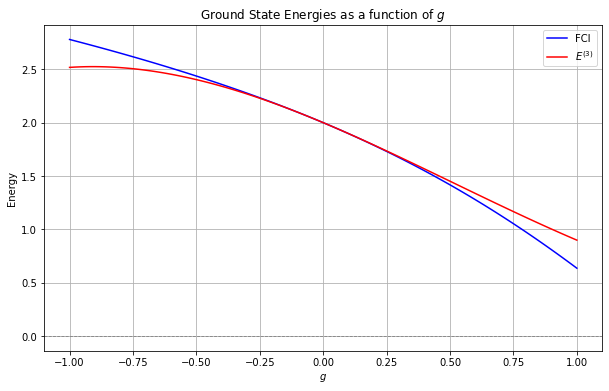
\includegraphics[width=0.6\linewidth]{exc5_3.png}
    \caption{$E^{(3)}$ compared to FCI}
    \label{fig:enter-label}
\end{figure}
We perform better than HF, as expected, but we still see poor performance in the 'extremes' of the $g$ range. One interesting thing to note is that $E^{(3)}$ is less than FCI for small $g$, whereas it is bigger for large $g$. This is even easier to see for the difference plot:
\begin{figure}[ht!]
    \centering
    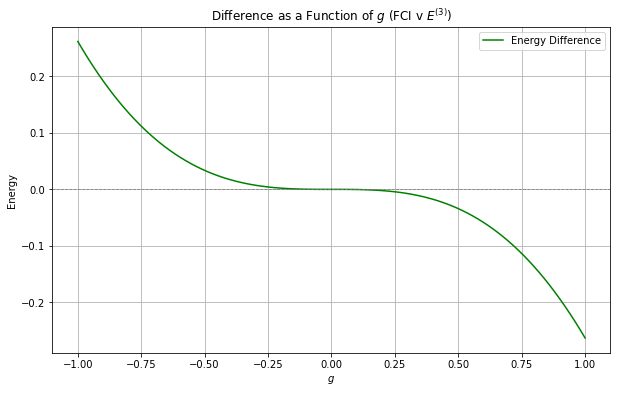
\includegraphics[width=0.6\linewidth]{exc5_4.png}
    \caption{Difference between FCI and $E^{(3)}$}
    \label{fig:enter-label}
\end{figure}
\newline
We see a characteristic $-x^3$ shape for the difference. Of our non-linear methods, this is by far the biggest error we've seen until now.
\newpage
\section{}
We designate a operator $\chi^{(1)}$, which is the first order wave operator, defined as:
\begin{equation*}
    \chi^{(1)}|\Phi_0\rangle = \sum_{p} \sum_{q} |\Phi_p^\sigma \rangle \frac{\langle \Phi_{p q}^{\sigma_p \sigma_q} | \hat V | \Phi_0 \rangle}{E^{(0)} - E_{p\sigma}^{(0)}} \delta(\sigma_p, \sigma_q)
\end{equation*}
which is (as shown by the Kronecker delta) only valid for states where the the spins are opposite. \newline
The second order contributions are simply written as:
\begin{equation*}
    E^{(2)} = \sum_p \frac{\langle \Phi_0 | \hat V | \Phi_p \rangle \langle \Phi_p | \hat V | \Phi_0 \rangle}{\langle \Phi_p | \hat H_0 | \Phi_p \rangle - \langle \Phi_0 | \hat V | \Phi_0 \rangle}
\end{equation*}
from which we get:
\begin{equation*}
    E^{(2)} = \sum_{ia} \frac{\langle i_+ i_- | \hat V | a_+ a_- \rangle_{AS} \langle a_+a_-| \hat V | i_+ i_- \rangle_{AS}}{2\epsilon_a - 2\epsilon_i}
\end{equation*}
\newline
I am not entirely sure about what to do from here in regards to comparing our results with those of problem 3), so this has been left out.
\section{}
We can immediately off the bat disregard \emph{1p1h} as they are not paired, thus not fitting with our Hamiltonian.\newline
We have then the \emph{2p2h} diagrams. It is hard to make out exactly what contributes, as they all look \emph{very} much alike. As such, I am going to be guessing for these. We note that $5, 6$ and $14, 15$ are the only diagrams mirrored along the $y$-axis, for lack of a better term. Therefore, we choose these.
\newline
For \emph{3p3h}, I believe can again disregard these as they are incompatible with our Hamiltonian, though I am not certain. \newline
For \emph{4p4h}, we have first the most obvious ones, $36$ and $37$. We secondly have the unlinked diagrams $33$ and $41$. According to the linked diagram, we can disregard the contributions of $33$ and $41$, as their contributions are typically a product of lower-order diagrams (that is to say that they factorize into products of lower-order diagrams). \newline
Because of this, we only need to look at a total of six diagrams, $5_2, 6_2, 14_2, 15_2, 36_4$ and $37_4$, the subscript indicating which series of diagrams they belong to. \newline
From here, we try the same approach as we did in problem 5, but we note that as all these are symmetric, we only need to calculate three, then change the indices to get it's opposite. We have:
\begin{equation*}
    (5) \; \; \; \; \frac{1}{128} \sum_{acik} \frac{g^4}{(i-a)(k-a)(k-c)} \xrightarrow[]{} (6)\;\;\;\; \frac{1}{128} \sum_{acik} \frac{g^4}{(i-a)(i-c)(k-c)}
\end{equation*}
\begin{equation*}
    (14) \;\;\;\; \frac{1}{128} \sum_{acei} \frac{g^4}{(i-a)(i-c)(i-e)} \xrightarrow[]{} (15) \;\;\;\; \frac{1}{64} \sum_{acei} \frac{g^4}{(i-a)(i-a)(m-a)}
\end{equation*}
\begin{equation*}
    (36) \;\;\;\; \frac{1}{128} \sum_{acik} \frac{g^4}{(i-a)(i+k-a-c)(i-c)} \xrightarrow[]{} (37) \; \; \; \; \frac{1}{128} \sum_{acik} \frac{g^4}{(i-a)(i+k-a-c)(k-a)}
\end{equation*}
Summing this is tedious and ultimately a very pointless exercise (just know that the procedure is the same as in the latter half of  5)), so we leave it to Python, and find the following plot when varying $g$:
\newline
\begin{figure}[ht!]
    \centering
    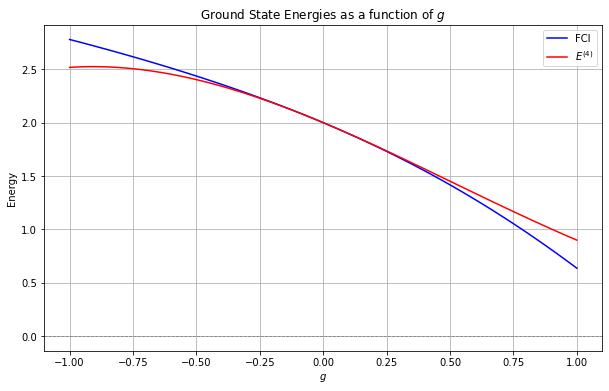
\includegraphics[width=0.6\linewidth]{exc7_1.png}
    \caption{Difference between FCI and $E^{(4)}$}
    \label{fig:enter-label}
\end{figure}
\newline
which is a (albeit small) change from $E^{(3)}$. This is quite hard to see, so we (instead of looking at the usual difference between FCI and whatever method we're studying) look at the absolute difference between the differences. That is to say, we first look at the difference between $E^{(3)}$ and FCI, then ditto for $E^{(4)}$. We then compare those differences to each other, which is:
\begin{figure}[ht!]
    \centering
    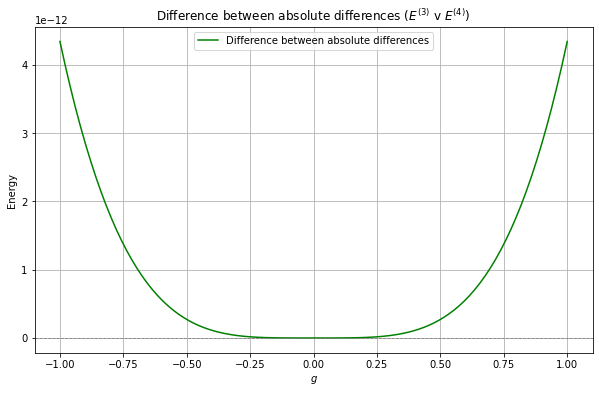
\includegraphics[width=0.6\linewidth]{exc7_3.png}
    \caption{Absolute difference between $E^{(3)}$ and $E^{(4)}$}
    \label{fig:enter-label}
\end{figure}
\newline
This result is not entirely unexpected. After all, increasing the order of our energy corrections is not necessarily a guarantee that it will perform better (or worse) than previously.
\newpage
Lastly, we decide to look all the methods discussed in this midterm in one final plot, as a 'summary' of our work:
\begin{figure}[ht!]
    \centering
    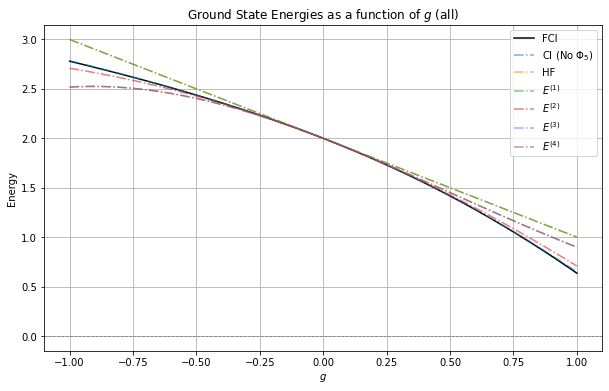
\includegraphics[width=0.6\linewidth]{exc7_4.png}
    \caption{All the methods discussed in this midterm on one single plot}
    \label{figall}
\end{figure}
We see here that, ultimately, the margin between \emph{most} of the methods are very small to non-existent for any $g$ in the $\{-0.5, 0.5\}$ range. We can further study this by blowing up our plot:
\begin{figure}[ht!]
    \centering
    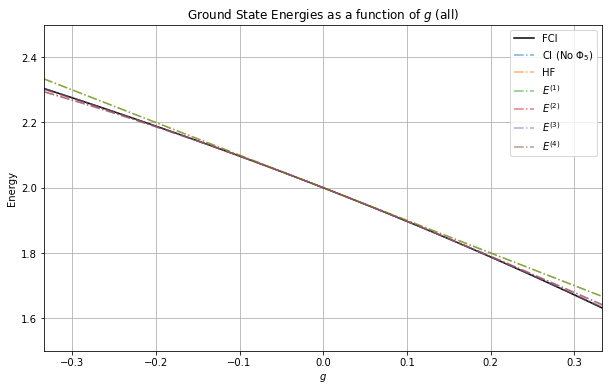
\includegraphics[width=0.6\linewidth]{exc7_5.png}
    \caption{A zoomed in version of Figure \ref{figall}}
    \label{fig:enter-label}
\end{figure}
which as we can see, further emphasizes the margins of many of our studied methods.
\newline
\end{document}
